\chapter{Related work}

In the introduction, we presented the programming language C\# and its possible improvement of type inference. 
This chapter continues by describing relevant sections of the C\# language and its type inference algorithm to understand the possible barriers to implement improved type inference. 
As a primary source of inspiration for the improvement, we will explore Hindley-Milner type inference in more detail and describe its modification in Rust and C\# programming languages. 
For the third goal of this thesis, we will mention relevant C\# language issues presented on the GitHub repository, which we use later to prioritize the improvement features to make it more likely to be accepted by \ac{LDM}. 

\section{C\# programming language}

\info{Explain purpose of this section}
Although C\# language features complement each other, we try to extract only relevant components for type inference in this section. 
We describe the type system, including C\# generics and their possibilities. 
Then, we mention unrelated language constructs that influence the type inference, and we have to count on them in proposing improved type inference. 
At the end of this section, we list types of type inference in C\# and describe them in necessary detail for the following chapters.

\subsection{Type system}

\info{Value/reference types}
\info{Inheritance}
As we mentioned in the introduction, each variable and expression returning a value has to have a type in the C\# type system \cite{online:cSharpTypeSystem} called the \ac{CTS}.
Its fundamental characteristic is type inheritance, where every type directly or indirectly inherits a base type \texttt{System.Object}, as you can see in the picture \ref{img04:typeSys}.
This chain of inheritance forms a tree, meaning that it is prohibited to inherit more than one type.
Types are divided into value and reference types.
Value types consist of built-in numeric types, structures (\texttt{struct}), and enumeration (\texttt{enum}).
Compared to classes (\texttt{class}) and records (\texttt{record}) belonging to reference types, value types can't be inherited by other types.
The last relevant member of reference types is interface (\texttt{interface}), which can extend multiple interfaces and be implemented by \texttt{class}, \texttt{record}, or \texttt{struct}.
\par
\begin{figure}[b!]
\centering
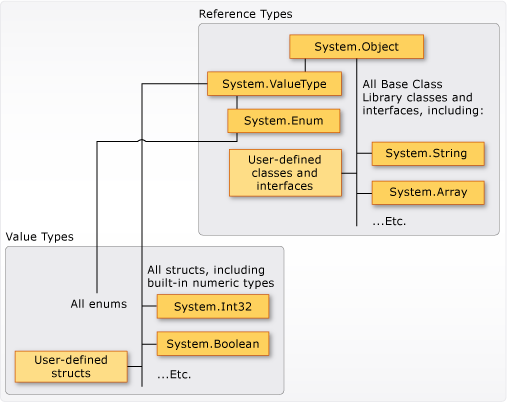
\includegraphics[width=140mm, height=100mm]{../img/value-reference-types-common-type-system.png}
\caption{The C\# type system \cite{online:cSharpTypeSystem}.}
\label{img04:typeSys}
\end{figure}
\par
\info{Nullability analysis}
C\# type inference infers, besides a type, its nullability, determining if it is possible to assign \texttt{null} value to that type.
C\# implicitly allows to assign \texttt{null} values to reference types indicating invalid value.
Since C\# 2.0 \cite{online:csHist}, it allows to assign \texttt{null} values to nullable value types, which are generic wrappers around value types.
Because assigning \texttt{null} value is referred to as a billion-dollar mistake, C\# 8.0 introduces optional settings prohibiting it and created nullable reference types explicitly allowing \texttt{null} assignment as a way of interaction with legacy code not using the feature.
\par
\info{Generic types and methods}
An essential part of the type system is C\# Generics, allowing parametrization of types and methods by other types. 
An example of a generic class is \texttt{System.Collections.Generic.List<T>} representing resizeable mutable array where  \texttt{T} represents arbitrary data type, which we want to have a collection of. 
Providing a type argument for  \texttt{T}, we create a new type where the type argument replaces the usages of  \texttt{T}.
\par
\info{Generic constraints}
Because a type parameter can be arbitrary, C\# treats it as a \texttt{System.Object}, which is insufficient in cases where the type parameter should provide special behaviour distinct from \texttt{System.Object}.
This requirement is achieved by type constraints, which restrict a set of types that can be passed to the parameter.
Several types of restrictions can be applied to type parameters in order to enable more actions on values of the restricted type parameters.
We can see examples of type constraints in the following code \ref{img05:typeConst}, where we use implementation restriction forcing the \texttt{T} to implement an interface providing API for comparing values with the same type.
The second restriction forces the type argument to have a default constructor.
Another restriction concerns an obligation that the type will be a value type or the type has to be non-nullable.
\par
\begin{figure}
\begin{lstlisting}[style=csharp]
class MyList<T> : where T : IComparable<T>, new()
{  
	private T[] myBuffer;
	
	int CompareOnIndicies(int idx1, int idx2) {
		return myBuffer[idx1].CompareTo(myBufffer[idx2])	
	}
}
\end{lstlisting}
\caption{C\# type constraints.}
\label{img05:typeConst}
\end{figure}
\par
\info{Variance and contra-variance}
The last feature of generics influencing type inference is the concept of type variance.
Initially, type parameters are invariant, meaning an obligation to assign a generic type to another generic type having the same types of type parameters.
Generic interfaces introduce additional modifiers (\texttt{in}, and \texttt{out}) of type parameters, which allow to assign a type with the more specialized type argument to a type with the less specialized type argument or vice-versa respectively.
\par
\info{Overloading}
We end this subsection by presenting method overloading. 
C\# allows the definition of multiple methods with the same and count of type arguments having different parameters. 
We will see in the following chapters why this feature is one of the barriers to implement strong and efficient type inference.

\subsection{Relevant constructs}

\info{Dynamic}
C\# type inference mostly happens at compile time, with one exception. 
We previously mentioned that C\# requires knowing the types of all variables and expressions during compilation. 
It turned out that the possibility of expressing type, which is unknown at compile time, became crucial for interoperability with other dynamic typed languages. 
To make the interoperability easier, C\# introduced a dynamic keyword that can be used as an ordinary type, which causes late binding. 
Internally, the type is \texttt{System.Object}, however, the compiler skips its binding and postpones it to the runtime. 
This feature creates the exception when type inference happens at runtime, although the compiler still attempts to check expressions containing dynamic values to reveal possible errors. 
This process will be explained in the following section.
\unsure{Code example}
\par
\info{Implicit typed lambdas}
The next language construct influencing type inference is an anonymous function, also known as Lambda, which, instead of declaring a dedicated method with a signature and a body, allows to specify only the body with untyped parameters on places where a function delegate is required. 
Type inference infers its signature based on the surrounding context.
\unsure{Code example}
\par
\info{Object creation expression and initializers}
The last language feature which will take part in the improved type inference are initializers used as a shortcut during an object instantiation.
The most simple one is an object initializer that allows to assign values to the object's fields in a pleasant way instead of assigning them separately after the initialization.
The second type of initializers regard arrays and collections.
Array initializers are used to create fixed arrays with predefined content.
Under the hood, each of the items in the initializer is assigned to the corresponding index of the array after the array creation.
Collection initializers are similar to an array initializer defined on collections which are determined by implementing \texttt{ICollection<T>} interface.
One of the interface's declaring methods is \texttt{void Add<T>(T)} with adding semantic.
Each type implementing this interface is allowed to use an initializer list in the same manner as an array initializer.
It's just a sugar code hiding to call the `Add` method for each item in the initializer list.
The last type of initializer uses indexer to store referred values on predefined positions.
\unsure{Code example}

\subsection{Type inference}

\info{Introduce kinds of type inferences}
\info{Method type inference}
C\# type inference occurs in many contexts. 
However, we mention only these related to our improvement described in the following sections. 
One of the most simple occurrences regards the \texttt{var} keyword, which is used in the variable declaration, as we can see in code \ref{img09:var}. It lets the compiler decide the type of variable based on the type of initializing value, which implies that we can’t use the keyword in declarations without initializing the value.
\par
\begin{figure}
\begin{lstlisting}[style=csharp]
var myVariable = "string";
\end{lstlisting}
\caption{\texttt{var} keyword}
\label{img09:var}
\end{figure}
\par
The most interesting and complex context is the method type inference used during generic method call binding when type arguments are not given. 
We can see a situation when the method type inference deduces \texttt{System.String}, \texttt{System.Int32} and \texttt{System.Int32} as type arguments of the \texttt{MyMethod} method in the following code \ref{img06:typeInference}. 
We can notice several tasks that the type inference has to be capable of.
Regarding the \texttt{T1} type parameter, the inference has to find a common type between the first and the second type parameters. 
Regarding the \texttt{T2} type parameter, the type inference has to go into type arguments of the generic type of parameter and the argument, check if the types are compatible, and then match the type parameter against the type argument of the third parameter. 
The most challenging is lamdas, whose return type has to be inferred after all lambda argument types are inferred.
\par
\begin{figure}
\begin{lstlisting}[style=csharp]
Helper.MyMethod((long)1, 1, new List<int>(), (p1) => p1 + 1);

class Helper {
  static void 
  MyMethod<T1, T2, T3>(T1 p1, T1 p2, IList<T2> p3, Func<T2,T3> p4) 
  { ... }
}
\end{lstlisting}
\caption{C\# Method type inference deduces the method type arguments.}
\label{img06:typeInference}
\end{figure}
\par
As we can see, the method type inference is a complex process containing many steps.
Since one of our improvement is adjusting the algorithm, we present its complete description.
The algorithm is divided into four sections to better explain its functionality.
Before we show schema, we have to present definitions which are used by the algorithm.
\par
\unsure{Create citations}
\begin{defn}[Fixed type variables, bounds]
We call inferred type parameters \emph{type variables} which are at the beginning of the algorithm unknown, \emph{unfixed}. 
During the algorithm, they start to be restricted by sets of \emph{bounds}.
The type variable becomes \emph{fixed} when the its actual type is determined using its \emph{bounds}.
\end{defn}
\begin{defn}[Input/Output types]
If \texttt{E} is a method group or anonymous function and \texttt{T} is a delegate or expression tree type, then return type of \texttt{T} is an \emph{output type} of \texttt{E}.
If \texttt{E} is a method group or implicitly typed anonymous function, then all the parameter types of \texttt{T} are \emph{input types} of \texttt{E}. 
\end{defn}
\par
\begin{defn}[Dependence]
An unfixed type variable \texttt{$X_i$} \emph{depends directly on} an unfixed type variable \texttt{$X_e$} if for some argument \texttt{E} \texttt{$X_e$} occurs in an input type of \texttt{E} and \texttt{$X_i$} occurs in an output type of \texttt{E}.
\texttt{$X_i$} \emph{depends on} \texttt{$X_e$} is the transitive but not reflexive closure of \emph{depends directly on}.
\end{defn}
\par
\info{Algorithm description}
Method type inference process starts with receiving arguments of a method call and the method's signature which type parameters has to deduce as we can see in the first schema \ref{alg01:methodTypeInference1}.
The algorithm has two phases where the first phase initializes initial bounds' sets of type variables(inferred type arguments) and the second phase repeats until all type variables are fixed or fails if there is not enough information to deduce it.
Each type variable has three type of bounds. 
Exact bound consists of types which has to be identical to the type variable meaning that they can convert to each other.
Lower bound contains types which has to be convertible to the type variable and Upper bound is opposite to it.
\info{The first phase description}
The first phase iterates over provided arguments and chooses the right set where to add the type of the argument by calling helper functions based on several conditions.
We suppose the reader has knowledge of C\# language so we quickly mention used functions contained in the conditions for clarifying meant constructs of parameters and arguments.
\texttt{isValParam()} and \texttt{isRefParam()} functions determine if the parameter is passed by value or by reference.
There are also \texttt{isInParam()}, \texttt{isOutParam()}, \texttt{isInArg()} referring to use of \texttt{in} and \texttt{out} keyword in parameter declarations and \texttt{in} keyword in argument position.
\info{The second phase description}
The second phase happens iteratively respecting \textit{depends on} relation.
Each iteration has two goals.
The first one is fixation of at least one type variable.
If there is no type variable to fix because either all type variables are fixed or there are no other type bounds which could be used for type variable deduction, the phases and algorithm ends.
The sets \texttt{$X_{indep}$} and \texttt{$X_{dep}$} referring to type variables, which can be fix in the current iteration.
Line 24 contains a case ending the algorithm when all type variables are fixed or there is no way how to infer next ones.
The second goal checks for output types, which where dependent on input types where the last unfixed types were fixed in this iteration, and infers them.
We can see respecting order of inferring return type of anonymous functions at line 29 where we are inferring return type of lambdas when all type variables contained in parameter list are fixed.
\par
\begin{algorithm}
\SetKwFunction{FirstPhase}{FirstPhase}
\SetKwFunction{SecondPhase}{SecondPhase}
\SetKwFunction{InferExplicitParameterType}{InferExplicitParameterType}
\SetKwFunction{InferExact}{InferExact}
\SetKwFunction{InferLowerBound}{InferLowerBound}
\SetKwFunction{isValueParameter}{isValParam}
\SetKwFunction{isReferenceParameter}{isRefParam}
\SetKwFunction{isInputParameter}{isInParam}
\SetKwFunction{isInputArgument}{isInArg}
\SetKwFunction{isOutputParameter}{isOutParam}
\SetKwFunction{Fix}{Fix}
\SetKwFunction{Failed}{Failed}
\SetKwFunction{Return}{Return}
\SetKwFunction{inputTypes}{inTypes}
\SetKwFunction{outputTypes}{outTypes}
\SetKwFunction{GoTo}{GoTo}
\SetKwFunction{InferOutputType}{InferOutputType}
\SetKwProg{Fn}{fn}{:}{}

\KwIn{a method call \texttt{M($\mathtt{E_1, ..., E_x}$)} and its signature \texttt{$\mathtt{T_e}$ M<$\mathtt{X_1, ..., X_n}$>($\mathtt{T_1 p_1, ..., T_x p_x}$)}}
\KwOut{$X_1, ..., X_n$}
$B_{lower}, B_{upper}, B_{exact}, F \gets [\ ]$\;
\FirstPhase{}\;
\SecondPhase{}\;
\Fn{\FirstPhase{}}{
	\ForEach{$E_i$}{
		\If{$E_i$ $\in$ AnonymousFuncs}{
			\InferExplicitParameterType{$E_i, T_i$}
		}
		\ElseIf{$E_i$ has a type $U$}{
			\Switch(\tcc*[h]{At most one case is executed}){$U$}{
				\lCase{\isValueParameter{$p_i$}}{\InferLowerBound($U, T_i$)}
				\Case{\isReferenceParameter{$p_i$} $\vee$ \isOutputParameter{$p_i$}}{\InferExact{$U, T_i$}}
				\Case{\isInputParameter{$p_i$} $\wedge$ \isInputArgument{$E_i$}}{\InferExact{$U, T_i$}}
				\lCase{\isInputParameter{$p_i$}}{\InferLowerBound{$U, T_i$}}
			}
		}
	}
}
\Fn{\SecondPhase{}}{
	$X_{indep} \gets \forall X_i : F[i] = null \wedge \nexists X_e : dependsOn(X_i, X_e)$\;
	$X_{dep} \gets \forall X_i\ :\ F[i] = null\ \wedge (\exists X_e : dependsOn(X_e, X_i) \vee B_{lower}[i] \cup B_{exact}[i] \cup B_{upper}[i] \neq empty)$\;
	\Switch{$X_{indep}$, $X_{dep}$}{
		\Case{$X_{indep}$ $\neq$ empty}{
			\lForEach{$X_s$ $\in$ $X_{indep}$}{\Fix{$X_s$}}		
		}
		\Case{$X_{indep}$ = empty $\wedge$ $X_{dependent}$ $\neq$ empty}{
			\lForEach{$X_s$ $\in$ $X_{indep}$}{\Fix{$X_s$}}				
		}
		\Case{$X_{indep}$ $\cup$ $X_{dep}$ = empty}{
		\lIf{$\exists X_k$ : F[k] = null}{\Failed{}}
		\lElse{\Return{F[0], ..., F[n]}}
		}
		\Other{
			\lForEach{$E_i$ : $\exists$ $X_e$ : F[e] = null $\wedge$ $X_e$ $\in$  \outputTypes{$T_i$} $\wedge$ $\nexists$ $X_k$ : F[k] = null $\wedge$ $X_k$ $\in$ \inputTypes{$T_i$}}{
				\InferOutputType{$E_i, T_i$}			
			}	
			\GoTo{\normalfont\texttt{16}}	
		}
	}
}
\caption{Phases of Method Type Inference}
\label{alg01:methodTypeInference1}
\end{algorithm}
\par
\change{Describe infer output type, infer explicit parameter type}
\par
\begin{algorithm}
\SetKwFunction{OverloadResolution}{OverloadResolution}
\SetKwFunction{InferOutputType}{InferOutputType}
\SetKwFunction{InferExplicitParameterType}{InferExplicitParameterType}
\SetKwFunction{InferReturnType}{InferReturnType}
\SetKwFunction{InferExact}{InferExact}
\SetKwFunction{InferLower}{InferLower}
\SetKwFunction{Add}{Add}
\SetKwProg{Fn}{fn}{:}{}

\Fn{\InferOutputType{E, T}}{
	\Switch{E}{
		\Case{E $\in$ AnonymousFuncs $\wedge$ T $\in$ DelegateTypes $\cup$ ExprTreeTypes}{
			\InferLower{\InferReturnType{E}, T.ReturnType}		
		}
		\Case{E $\in$ MethGroups $\wedge$ T $\in$ DelegateTypes $\cup$ ExprTreeTypes}{
			$T_{ret}, T_1,...T_n \gets T.ReturnType, T.ParamTypes$\; 
			$E_{resolved}$ $\gets$ \OverloadResolution{$E, T_1,...T_n$}\;
			\If{$\|E_{resolved}\|$ = 1}{
				\InferLower{$E_{resolved}[1].ReturnType, _{ret}$}			
			}
		}
		\lCase{E $\in$ Expressions $\wedge$ E has a type U}{
			\InferLower{U, T}
		}	
	}
}
\Fn{\InferExplicitParameterType{E, T}}{
	\If{E $\in$ ExplicitlyTypedAnonymousFuncs $\wedge$ T $\in$ DelegateTypes $\cup$ ExprTreeTypes $\wedge$ $\|E.ParamTypes\| = \|T.ParamTypes\|$}{
		\ForEach{$U_i, V_i$ : $U_i$ $\in$ E.ParamTypes $\wedge$ $V_i$ $\in$ T.ParamTypes}{
			\InferExact{$U_i, V_i$}		
		}	
	}
}
\Fn{\InferExact{U, V}}{
	\lIf{$\exists$ i : V = $X_i$ $\wedge$ F[i] = null }{
		$B_{exact}[i]$.\Add{U}	
	}
	\Switch{V}{
		\Case{V = $V_1$[...] $\wedge$ U = $U_1$[...] $\wedge$ V.Rank = U.Rank}{
			\InferExact{$U_1, V_1$}		
		}
		\lCase{V = \normalfont\texttt{$V_1$?} $\wedge$ U = $U_1$}{
			\InferExact{$V_1, U_1$}		
		}
		\Case{V = \normalfont\texttt{C<$V_1,...V_e$>} $\wedge$ U = \normalfont\texttt{C<$U_1,...U_e$>}}{
			\lForEach{$V_i, U_i$}{
				\InferExact{$V_i, U_i$}
			}		
		}
	}	
}
\caption{\textit{Output type inference}, \textit{Explicit parameter type inference}, \textit{Exact inference}}
\label{alg02:methodTypeInference2}
\end{algorithm}
\par
\change{Describe infer exact, lower, upper}
\par
\begin{algorithm}
\SetKwFunction{InferExact}{InferExact}
\SetKwFunction{InferLower}{InferLower}
\SetKwFunction{InferUpper}{InferUpper}
\SetKwFunction{isReferenceType}{isRefType}
\SetKwFunction{Add}{Add}
\SetKwFunction{IdenticalTo}{IdenticalTo}
\SetKwFunction{Inherits}{Inherits}
\SetKwFunction{Implements}{Implements}
\SetKwFunction{isCovariant}{isCovariant}
\SetKwFunction{isContravariant}{isContravariant}
\SetKwFunction{isInvariant}{isInvariant}
\SetKwProg{Fn}{fn}{:}{}


\Fn{\InferLower{U, V}}{
	\lIf{$\exists$ i : V = $X_i$ $\wedge$ F[i] = null }{
		$B_{lower}[i]$.\Add{U}	
	}
	\Switch{V, U}{
		\lCase{V = \normalfont\texttt{$V_1$?} $\wedge$ U = \normalfont\texttt{$U_1$?}}{
			\InferLower{$V_1, U_1$}		
		}
		\Case{V = $V_1$[...] $\wedge$ U = $U_1$[...] $\wedge$ V.Rank = U.Rank}{
			\lIf{\normalfont\texttt{!}\isReferenceType{$U_1$}}{
				\InferExact{$U_1$, $V_1$}		
			}
			\lElse{
				\InferLower($U_1$, $V_1$)			
			}
		}
		\Case{V $\in$ \{\normalfont\texttt{IEnumerable<$V_1$>}, \normalfont\texttt{ICollection<$V_1$>}, \normalfont\texttt{IReadOnlyCollection<$V_1$>}, \normalfont\texttt{IReadOnlyCollection<$V_1$>}, \normalfont\texttt{IList<$V_1$>}\} $\wedge$ U = $U_1$[ ]}{
			\lIf{\isReferenceType{$U_1$}}{
				\InferExact{$U_1$, $V_1$}		
			}
			\lElse{
				\InferLower($U_1$, $V_1$)			
			}
		}
		\Case{V = \normalfont\texttt{C<$V_1, ..., V_e$>} $\wedge$ $\exists!$ \normalfont\texttt{C<$U_1, ..., U_e$>} : \IdenticalTo{U, \normalfont\texttt{C<$U_1, ..., U_e$>}} $\vee$ \Inherits{U, \normalfont\texttt{C<$U_1, ..., U_e$>}} $\vee$ \Implements{U, \normalfont\texttt{C<$U_1, ..., U_e$>}}}{
			\Switch{${V_i}$}{
				\lCase{\isCovariant{${V_i}$}}{
					\InferLower{${U_i}$, ${V_i}$}
				}
				\lCase{\isContravariant{${V_i}$}}{
					\InferUpper{${U_i}$, ${V_i}$}
				}
				\lCase{\isInvariant{${V_i}$}}{
					\InferExact{${U_i}$, ${V_i}$}
				}			
			}
		}
	}
}
\Fn{\InferUpper{U, V}}{
	\lIf{$\exists$ i : V = $X_i$ $\wedge$ F[i] = null }{
		$B_{upper}[i]$.\Add{U}	
	}
	\Switch{V, U}{
		\Case{V = \normalfont\texttt{$V_1$?} $\wedge$ U = \normalfont\texttt{$U_1$?}}{
			\lIf{\normalfont\texttt{!}\isReferenceType{$U_1$}}{
				\InferExact{$U_1$, $V_1$}		
			}
			\lElse{
				\InferUpper($U_1$, $V_1$)			
			}
		}
		\Case{V = $V_1$[...] $\wedge$ U = $U_1$[...] $\wedge$ V.Rank = U.Rank}{
			\lIf{\normalfont\texttt{!}\isReferenceType{$U_1$}}{
				\InferExact{$U_1$, $V_1$}		
			}
			\lElse{
				\InferUpper($U_1$, $V_1$)			
			}
		}
		\Case{U $\in$ \{\normalfont\texttt{IEnumerable<$U_1$>}, \normalfont\texttt{ICollection<$U_1$>}, \normalfont\texttt{IReadOnlyCollection<$U_1$>}, \normalfont\texttt{IReadOnlyCollection<$U_1$>}, \normalfont\texttt{IList<$U_1$>}\} $\wedge$ V = $V_1$[ ]}{
			\lIf{\isReferenceType{$U_1$}}{
				\InferExact{$U_1$, $V_1$}		
			}
			\lElse{
				\InferLower($U_1$, $V_1$)			
			}
		}
		\Case{U = \normalfont\texttt{C<$U_1, ..., U_e$>} $\wedge$ $\exists!$ \normalfont\texttt{C<$V_1, ..., V_e$>} : \IdenticalTo{V, \normalfont\texttt{C<$V_1, ..., V_e$>}} $\vee$ \Inherits{V, \normalfont\texttt{C<$V_1, ..., V_e$>}} $\vee$ \Implements{V, \normalfont\texttt{C<$V_1, ..., V_e$>}}}{
			\Switch{${U_i}$}{
				\lCase{\isCovariant{${U_i}$}}{
					\InferUpper{${U_i}$, ${V_i}$}
				}
				\lCase{\isContravariant{${U_i}$}}{
					\InferLower{${U_i}$, ${V_i}$}
				}
				\lCase{\isInvariant{${U_i}$}}{
					\InferExact{${U_i}$, ${V_i}$}
				}			
			}
		}
	}
}
\caption{\textit{Upper-bound inference}, \textit{Lower-bound inference}}
\label{alg02:methodTypeInference2}
\end{algorithm}
\par
\change{Fix}
\par
\begin{algorithm}
\SetKwFunction{IdenticalTo}{IdenticalTo}
\SetKwFunction{hasImplicitConversion}{hasImplicitConversion}
\SetKwFunction{Failed}{Failed}
\SetKwFunction{Fix}{Fix}
\SetKwProg{Fn}{fn}{:}{}

\Fn{\Fix{$X_i$}}{
	$U_{candidates} \gets B_{upper}[i] \cup B_{exact}[i] \cup B_{lower}[i]$\;
	\ForEach{U ${\in}$ $B_{exact}[i]$}{
		$U_{candidates}$ -= \{$U_r$ : $U_r$ $\in$ $U_{candidates}$ $\wedge$ \normalfont\texttt{!}\IdenticalTo{$U_r$, U}\}
	}
	\ForEach{U ${\in}$ $B_{lower}[i]$}{
		$U_{candidates}$ -= \{$U_r$ : $U_r$ $\in$ $U_{candidates}$ $\wedge$ \normalfont\texttt{!}\hasImplicitConversion{U, $U_r$}\}
	}
	\ForEach{U ${\in}$ $B_{upper}[i]$}{
		$U_{candidates}$ -= \{$U_r$ : $U_r$ $\in$ $U_{candidates}$ $\wedge$ \normalfont\texttt{!}\hasImplicitConversion{$U_r$, U}\}
	}
	\lIf{$\exists!$ V : V $\in$ $U_{candidates}$ $\wedge$ $\forall$ $U_e$ $\in$ $U_{candidates}$ : \hasImplicitConversion{$U_e, V$}}{
		F[i] = V
	}
	\lElse{
		Failed()
	}
}
\caption{Fixing of type variables}
\label{alg03:methodTypeInference3}
\end{algorithm}
\info{Array type inference}
The third type inference happens in array initializers when the type of the array should be deduced from the initializer list.
We can see an example of situation, when the type inference is used for determining \texttt{myArray} type in the following code \ref{img08:arrayTypeInference}.
The most specialized common type is just adjusted already mentioned type inference algorithm where is just one type parameter and all initializer items are lower bounds of that type variable.
\par
\begin{figure}
\begin{lstlisting}[style=csharp]
var myArray = new[] {new object(), "string"};
\end{lstlisting}
\caption{C\# Method type inference algorithm.}
\label{img08:arrayTypeInference}
\end{figure}
\par
\info{Target-typed inference}
The fourth type inference regards inference based on target type.
The example of these situations can be seen in the following example where we use target-typed \texttt{new()} operator allowing to skipping creating type which is provided by the target type, variable type in this case.
\par
\begin{figure}
\begin{lstlisting}[style=csharp]
List<int> myList = new();
\end{lstlisting}
\caption{Target-typed \texttt{new()} operator.}
\label{img09:targetTypeInference}
\end{figure}
\par
\info{Dynamic checking}
The last group what we have to mention is rather type checking than type inference.
As we mentioned in the previous section, \texttt{dynamic} keyword is used to enable late binding on the expression containing dynamic expression.
Because of late binding, the compiler can't check instance method calling at compile time to prevent type errors at runtime.
However, there are situations, where the compiler can partial type check expressions like method calls.
You can see a situation, where despite of late-binding there is an obvious error where we try to pass arguments with \texttt{System.Int32} and \texttt{System.String} types to parameters with the same type.
Method type inference as we presented doesn't allow to infer \texttt{System.Object} when at least one bound doesn't contains that type causing type inference error at runtime.
To prevent these situations, where error are not related to dynamic values, the compiler tries to infer the types ignoring the dynamic values.
In case of type conflicts in the variable's bounds, the error is announced at compile time instead of runtime.
\par
\begin{figure}
\begin{lstlisting}[style=csharp]
dynamic dynamicValue = null;
Helper.MyMethod(1, "string", dynamicValue);

class Helper {
 static
 void MyMethod<T1, T2>(T1 p1, T1 p2, T2 p3) 
  { ... }
}
\end{lstlisting}
\caption{Type inference with dynamic argument.}
\label{img010:dynamicChecking}
\end{figure}

\section{Roslyn}

\info{Intro}
The implementation of C\# type inference can be found in the Roslyn compiler, as open-source compiler of C\# and VisualBasic developed at GitHub repository.
In this section we present Roslyn's architecture to better understand the context and restrictions which we have to consider to be able to plug the improved type inference into the compiler.
\par
\change{Overview of compilation pipeline}
\change{Binder}
\change{OverloadResolution}
\change{MethodTypeInferrer}
\change{NullableWalker}
\change{Dynamic biding vs. runtime binding}

\section{Hindley-Millner type inference}

\change{Hindley-Millner type system}
\change{Set of rules}
\change{Restriction and possible extensions}

\section{Rust type inference}

\change{Rust type system}
\change{Type inference context}
\change{Type inference across multiple statement}
\change{Constructor type inference}

\section{Github issues}

\change{Mention related Github issues and csharplang repo.}
\change{Roslyn and csharplang repo}
\change{Proposal champions}
\change{Related issues}
